\section{Wybór metody badawczej i uzasadnienie}
\label{sec:wyborMetodyBadawczejIUzasadnienie}

\par Do oceny wyników zostanie zastosowanie porównanie wybranych wskaźników, obliczonych na podstawia analizy danych wyeksportowanych z systemów. Wybrane wskaźniki to:
\begin{itemize}
    \item średnia odległość rozważanego patrolu od miejsca incydentu w trakcie podejmowania decyzji,
    \item średnia odległość wybranego patrolu od miejsca incydentu w trakcie podejmowania decyzji,
    \item średni czas potrzebny na dotarcie do miejsca zdarzenia,
    \item ilość aktywnych incydentów w czasie.
\end{itemize}
Wskazują one efektywność w rozwiązywaniu incydentów. Szczególnie istotnym jest tutaj wskaźnik ilości aktywnych incydentów w czasie. Ponieważ jeżeli ich ilość ciągle się zwiększa, oznacza to, że system nie jest w stanie odpowiednio szybko ich rozwiązywać.

\par Aby prawidłowo ocenić wpływ danych kontekstowych na algorytm decyzyjny, tylko one, a konkretniej wagi im przypisane, podlegają manipulacji. Zmienne podlegające eksperymentom, zostały przedstawione w tabeli \ref{tab:zmiennePodlegająceEksperymentom}. Pozostałe ustawienia są stałe i zostały one przedstawione w tabelach \ref{tab:ustawieniaSymulacji} i \ref{tab:ustawieniaHqService}.

\begin{table}[H]
    \centering
    \begin{tabular}{|c|}
        \hline
        Nazwa zmiennej \\
        \hline
        \hline
         \texttt{EvenPatrolDistribution} \\
         \hline
         \texttt{DistanceWeight} \\
         \hline
         \texttt{SameDistrictWeight} \\
         \hline
         \texttt{InsufficientNumberOfPatrolsInDistrictWeight} \\
         \hline
    \end{tabular}
    \caption{Zmienne podlegające eksperymentom}
    \label{tab:zmiennePodlegająceEksperymentom}
\end{table}

\begin{longtable}{|p{0.5\linewidth} | p{0.5\linewidth}|} 
    \hline
     Ustawienie & Wartość \\
     \hline
     \hline
     \makecell[tl]{SimulationSettings.TimeRate} & 240 \\
     \hline
     \makecell[tl]{SimulationSettings.EndAfterSimulationTime} & 1.00:00:00 \\
     \hline
     \makecell[tl]{IncidentDirectorSettings\\.DangerLevelShootingChance\\.Low} & 0 \\
     \hline
     \makecell[tl]{IncidentDirectorSettings\\.DangerLevelShootingChance\\.Normal} & 0.02 \\
     \hline
     \makecell[tl]{IncidentDirectorSettings\\.DangerLevelShootingChance\\.High} & 0.1 \\
     \hline
     \makecell[tl]{IncidentDirectorSettings\\.DangerLevelMaxNumberOfIncidentPerDay\\.Low} & 5 \\
     \hline
     \makecell[tl]{IncidentDirectorSettings\\.DangerLevelMaxNumberOfIncidentPerDay\\.Normal} & 15 \\
     \hline
     \makecell[tl]{IncidentDirectorSettings\\.DangerLevelMaxNumberOfIncidentPerDay\\.High} & 30 \\
     \hline
     \makecell[tl]{PatrolDirectorSettings\\.NormalPatrolSpeed} & 50 \\
     \hline
     \makecell[tl]{PatrolDirectorSettings\\.EmergencyPatrolSpeed} & 80 \\
     \hline
\caption{Ustawienia symulacji}
\label{tab:ustawieniaSymulacji}
\end{longtable}

\begin{longtable}{|p{0.5\linewidth} | p{0.5\linewidth}|} 
    \hline
    Ustawienie & Wartość \\
    \hline
    \hline
    \makecell[tl]{DecisionServiceSettings\\.DangerLevelRequiredPatrollingPatrols\\.Low} & 0 \\
    \hline
    \makecell[tl]{DecisionServiceSettings\\.DangerLevelRequiredPatrollingPatrols\\.Normal} & 1 \\
    \hline
    \makecell[tl]{DecisionServiceSettings\\.DangerLevelRequiredPatrollingPatrols\\.High} & 2 \\
    \hline
    Ilość patroli & 20 \\
    \hline
\caption{Ustawienia stałe \emph{HQ Service}, \emph{HQ Agent} oraz patroli}
\label{tab:ustawieniaHqService}
\end{longtable}

\par Mapa Krakowa została wybrana, jako miejsce do przeprowadzenia eksperymentów. Dzielnicom zostały przydzielone poziomy niebezpieczeństwa. Są one przedstawione na grafice \ref{fig:districtDangerLevelMap}.

\begin{figure}
    \centering
    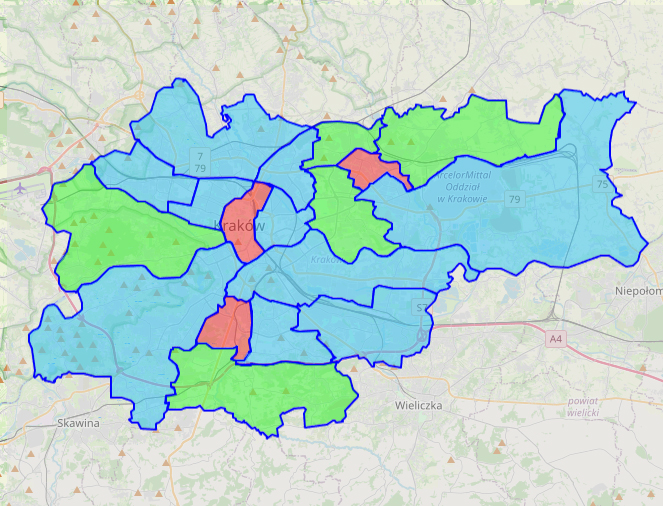
\includegraphics[width=\linewidth]{Districts - Danger Level Map}
    \caption{Kraków - dzielnice i ich poziomy niebezpieczeństwa. Zielony - \emph{Low}, Niebieski - \emph{Normal}, Czerwony - \emph{High}.}
    \label{fig:districtDangerLevelMap}
    \source{Opracowanie Własne}
\end{figure}

\par Aby zdobyć wiarygodną próbkę danych, każdą z konfiguracji postanowiono uruchomić trzykrotnie, a następnie obliczyć średnią z uzyskanych wyników. Decyzja ta została podjęta, aby ograniczyć błąd wynikający z niedeterministycznej natruy symulacji.